% Dokumentum konfiguráció
\documentclass[fleqn,12pt]{article}
% --------------------------------------------------
% Dokumentum adatok
% --------------------------------------------------

% Intézmény és kar
\newcommand\INTEZMENY{Budapesti Műszaki és Gazdaságtudományi Egyetem}
\newcommand\KAR{Gépészmérnöki Kar}
\newcommand\LOGO{bme-logo.jpg} % logo fájl neve a figures mappában

% Dokumentum adatok
\newcommand\CIM{Statik 4. Hausaufgabe}
\newcommand\DATUM{2025/26/1}
\newcommand\NEV{Abos Gergő}
\newcommand\NEPTUN{C46M9M}
\newcommand\EMAIL{gergo.abos@gmail.com}
\newcommand\TANTARGY{Statik}
\newcommand\TANTARGYKOD{BMEGEMMBXM1}

% --------------------------------------------------
% Preambulum és egyéni parancsok betöltése
% --------------------------------------------------

\input{../_settings/00_preambulum.tex}
\input{../_settings/01_commands.tex}
\input{../_settings/02_mechTikz.tex}
\usetikzlibrary{
  calc, % For coordinate calculations
  decorations.pathmorphing, % For support hatching
  patterns, % For filling (though not used here, opacity is)
  arrows.meta, % For arrow tips
  angles, quotes
}

% ==================================================
% Dokumentum kezdete
% ==================================================
\begin{document}

% Címlap és tartalomjegyzék
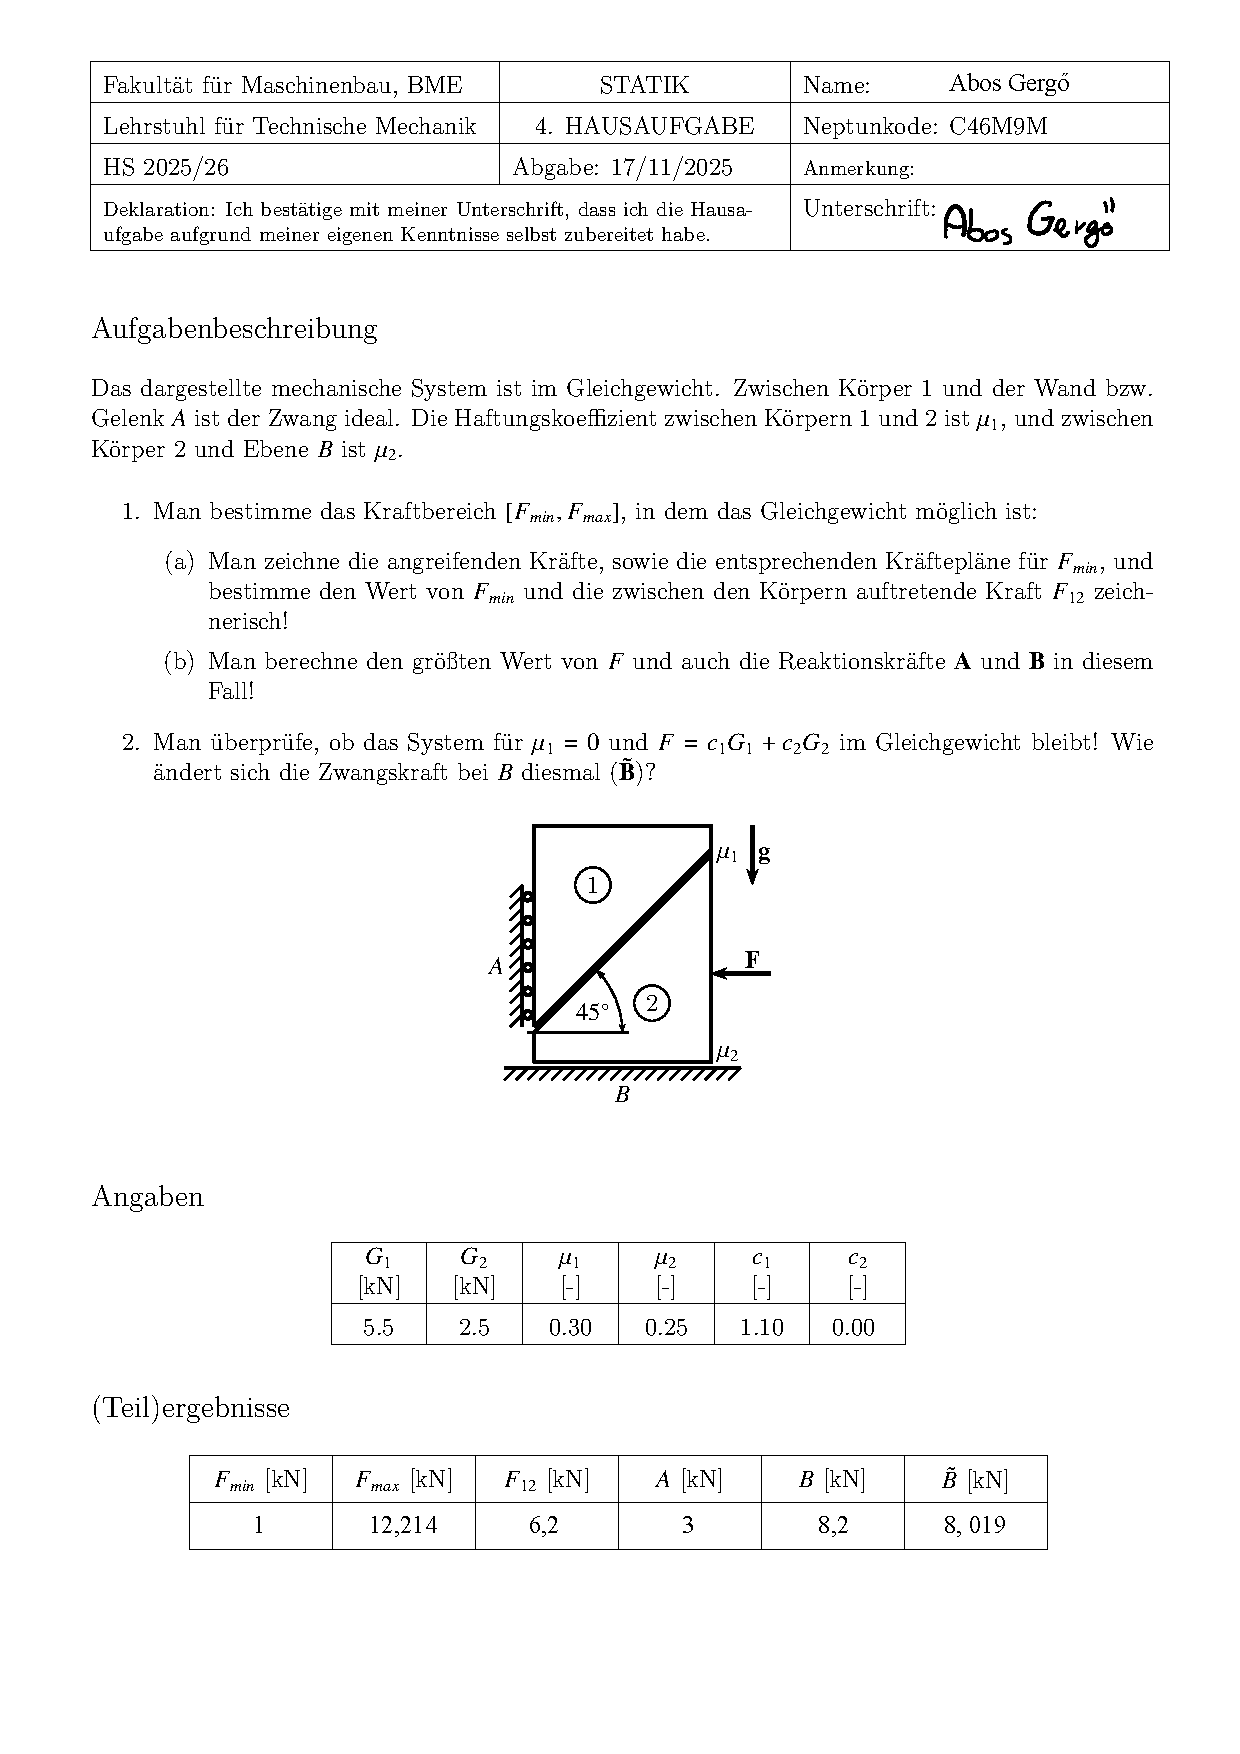
\includepdf[pages=1]{contents/stha4_filled.pdf}

\section[Kraftbereich Fmin bis Fmax]{Kraftbereich $[F_{\min}, F_{\max}]$}
\subsection[Mimimumwert von F zeichnerisch bestimmen]{Minimumwert von $F$ zeichnerisch bestimmen}
\label{sec:fmin}
Um den Minimalwert von $F$ zu bestimmen, geht man davon aus, dass das System kurz davor ist, sich zu bewegen. In diesem Grenzfall erreichen alle Reibkräfte, die der Bewegungsrichtung entgegenwirken, ihren maximalen Haftwert. Dadurch wird die Bewegung gerade noch verhindert und die benötigte äußere Kraft $F$ nimmt den kleinstmöglichen Wert an.

Die Haftungskraft kann Konstruktiert werden für Körper 1, dazu zeichne ich ein Freikörperbild.
\begin{figure}[H]
  \centering
  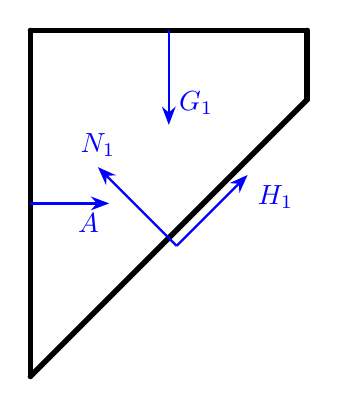
\begin{tikzpicture}[
      thick, % Default line thickness
      >=Stealth, % Default arrow tip
      force/.style={blue, very thick, ->}, % Style for force arrows
      dimline/.style={thin, <->, >=latex}, % Style for dimension lines
    ]

    % Größen
    \def\hone{0.5pt * 50}
    \def\htwo{2.5pt * 50}
    \def\w{2pt * 50}
    \def\fg{5.5pt * 2 / 3}
    \def\fa{4ptpt * 2 / 3}

    % Koordinaten von Punkte
    \coordinate (A) at (0, 0);
    \coordinate (B) at (\w, 0);
    \coordinate (C) at (\w, -\hone);
    \coordinate (D) at (0, -\htwo);

    % Starrkörper
    \foreach \i/\j in {A/B, B/C, C/D, D/A}
    \draw[line width=2pt, black, cap=round] (\i) -- (\j);

    % Gewichtskraft G1 (nach unten)
    \draw[force, thick] ($(A)!0.5!(B)$) -- ++(0,-1.2) node[above right] {$G_1$};

    % Kontaktkraft N12: normale zur 45°-Fläche
    % Richtung: von Körper 2 auf Körper 1 → wirkt nach oben-links
    \draw[force, thick] ($(C)!0.5!(D)$) + (0.1, -0.1) -- ++(-0.9,0.9)
    node[above] {$N_{1}$};

    % Reibkraft f12: tangential zur Fläche
    % Bei F_min wird Körper 2 nach links rutschen wollen, also wirkt Reibung auf 1 nach unten-rechts
    \draw[force, thick] ($(C)!0.5!(D)$) + (0.1, -0.1) -- ++(1., 0.8)
    node[below right] {$H_1$};

    % Reaktionskraft an der Wand A
    \draw[force, thick] ($(A)!0.5!(D)$) -- ++(1,0) node[below left] {$A$};
  \end{tikzpicture}
  \caption{Freikörperbild von Körper 1}
\end{figure}
Die Kraft $N_1$ (Normalkraft) und $H_1$ (Reibung) wird mit einer Kraft $W_{1}$ ersetzt. Die maximale Haftungswinkel von dieser Kraft kann mit der Haftungskoeffizient berechnet werden:
\begin{align*}
  \tan \alpha_{1} &= \mu_1\\
  \alpha_{1} &= 16,7^\circ
\end{align*}
Weil das Körper im Gleichgewicht sein muss, sollen die drei Kräfte ($G_1, A, W_{1}$) ein geschlossenes Dreieck bilden.
\begin{figure}[H]
  \centering
  \begin{tikzpicture}[
      thick, % Default line thickness
      >=Stealth, % Default arrow tip
      force/.style={blue, very thick, ->}, % Style for force arrows
      dimline/.style={thin, <->, >=latex}, % Style for dimension lines
    ]

    \def\fg{-5.5cm}

    % Gewichtskraft G1 (nach unten)
    \draw[force] (0, 0) -- (0, \fg) node[above right] {$G_1$};

    % Reaktionskraft an der Wand A
    \draw[force] (-2.96144cm,0) -- (0, 0) node[above left] {$A$};
    % WL von A
    \draw[dashed, blue] (-5, 0)-- (5, 0);

    \draw[thick] (1cm, \fg + 1cm) -- (-1cm, \fg -1cm);
    \draw[dashed] (-2cm, \fg + 2cm) -- (0, \fg);

    \draw[force] (0, \fg) -- ++(118.3:6.2466cm) node[below left] {$W_1$};

    \coordinate (C) at (-3cm, \fg + 3cm);
    \coordinate (B) at (0, \fg);
    \coordinate (A) at ($(0, \fg) + (118.3:3cm)$) node[below, xshift=-40pt, yshift=-94pt] {$\alpha_1$};
    \pic [draw, angle radius=2.8284cm] {angle = A--B--C};

  \end{tikzpicture}
  \caption{Geschlossenes Dreieck von Kräfte $G_1, A, W_{1}$}
\end{figure}
Von der Abbilgung kann die Größe der Kräfte $A$ und $W_{1}$ ablesen werden.
\begin{align*}
  &A = 3\text{ kN}\\
  &W_{1} = 6,2\text{ kN}
\end{align*}

Jetzt kann das Freikörperbild zum Körper 2 aufgezeichnet werden.
\begin{figure}[H]
  \centering
  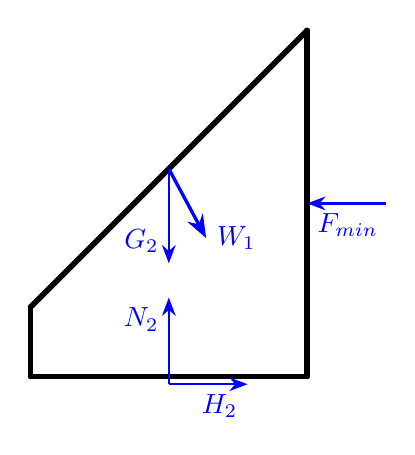
\begin{tikzpicture}[
      thick, % Default line thickness
      >=Stealth, % Default arrow tip
      force/.style={blue, very thick, ->}, % Style for force arrows
      dimline/.style={thin, <->, >=latex}, % Style for dimension lines
    ]

    % Größen
    \def\hone{0.5pt * 50}
    \def\htwo{2.5pt * 50}
    \def\w{2pt * 50}
    \def\fg{5.5pt * 2 / 3}
    \def\fa{4ptpt * 2 / 3}

    % Koordinaten von Punkte
    \coordinate (A) at (0, 0);
    \coordinate (B) at (\w, 0);
    \coordinate (C) at (\w, \htwo);
    \coordinate (D) at (0, \hone);

    % Starrkörper
    \foreach \i/\j in {A/B, B/C, C/D, D/A}
    \draw[line width=2pt, black, cap=round] (\i) -- (\j);

    \draw[force, thick] ($(D)!0.5!(C)$) -- ++(0,-1.2) node[above left] {$G_2$};

    \draw[force] ($(D)!0.5!(C)$) -- ++(298.3:1cm) node[right] {$W_1$};

    \draw[force, thick] ($(A)!0.5!(B)$) + (0, -0.1) -- ++(0, 1)
    node[below left] {$N_{2}$};

    \draw[force, thick] ($(A)!0.5!(B)$) + (0, -0.1) -- ++(1, -0.1)
    node[below left] {$H_2$};

    \draw[force, thick] ($($(B)!0.5!(C)$) + (1, 0)$) -- ++(-1,0) node[below right] {$F_{min}$};
  \end{tikzpicture}
  \caption{Freikörperbild von Körper 2}
\end{figure}
$N_2$ und $H_2$ wird auch mit ein Kraft $W_2$ ersetzt. Haftungswinkel kann wieder berechnet werden:
\begin{align*}
  \tan \alpha_{2} &= \mu_2\\
  \alpha_{2} &= 14,04^\circ
\end{align*}
Die vier Kräfte $G_2$, $W_1$, $W_2$, $F_{min}$ sollen im Gleichgewicht sein, also sie bilden ein geschlossenes Viereck.
\begin{figure}[H]
  \centering
  \begin{tikzpicture}[
      thick, % Default line thickness
      >=Stealth, % Default arrow tip
      force/.style={blue, very thick, ->}, % Style for force arrows
      dimline/.style={thin, <->, >=latex}, % Style for dimension lines
    ]

    \def\fg{-2.5cm}

    \def\fmin{-0.9601cm}

    % Gewichtskraft G1 (nach unten)
    \draw[force] (0, -\fg) -- (0, 0) node[above right] {$G_2$};

    % Reaktionskraft an der Wand A
    \draw[force] (0, 0) -- (\fmin,0) node[below] {$F_{min}$};
    % WL von A
    \draw[dashed, blue] (-5, 0)-- (5, 0);

    \draw[force] ($(0, -\fg) - (298.3:6.2466cm)$) -- (0, -\fg) node[above right] {$W_1$};

    \def\wtwo{8.246cm}
    \draw[force] (\fmin, 0) -- ++(104.04:\wtwo) node[below left] {$W_2$};

  \end{tikzpicture}
  \caption{Geschlossenes Viereck von Kräfte $G_2$, $W_1$, $W_2$, $F_{min}$}
\end{figure}
$W_2$ und $F_{min}$ können abgelesen werden.
\begin{align*}
  &W_{2} = 8,2\text{ kN}\\
  &\boxed{F_{min} = 1\text{ kN}}
\end{align*}

\subsection[Maximumwert von F berechnen]{Maximumwert von $F$ berechnen}
Wenn $F$ ein maximumwert $F_{max}$ beträgt, wirken alle Reibungskräfte maximal gegen dieser Kraft, alle $H_i$ Kräfte werden entgegen gesetzt sein als in \ref{sec:fmin}.

Die Haftungswinkel sind schon berechnet:
\begin{align*}
  \alpha_1 = 16,7^\circ\\
  \alpha_2 = 14,04^\circ\\
\end{align*}
Das Freikörperbild für Körper 1 kann wieder aufgezeichnet werden.
\begin{figure}[H]
  \centering
  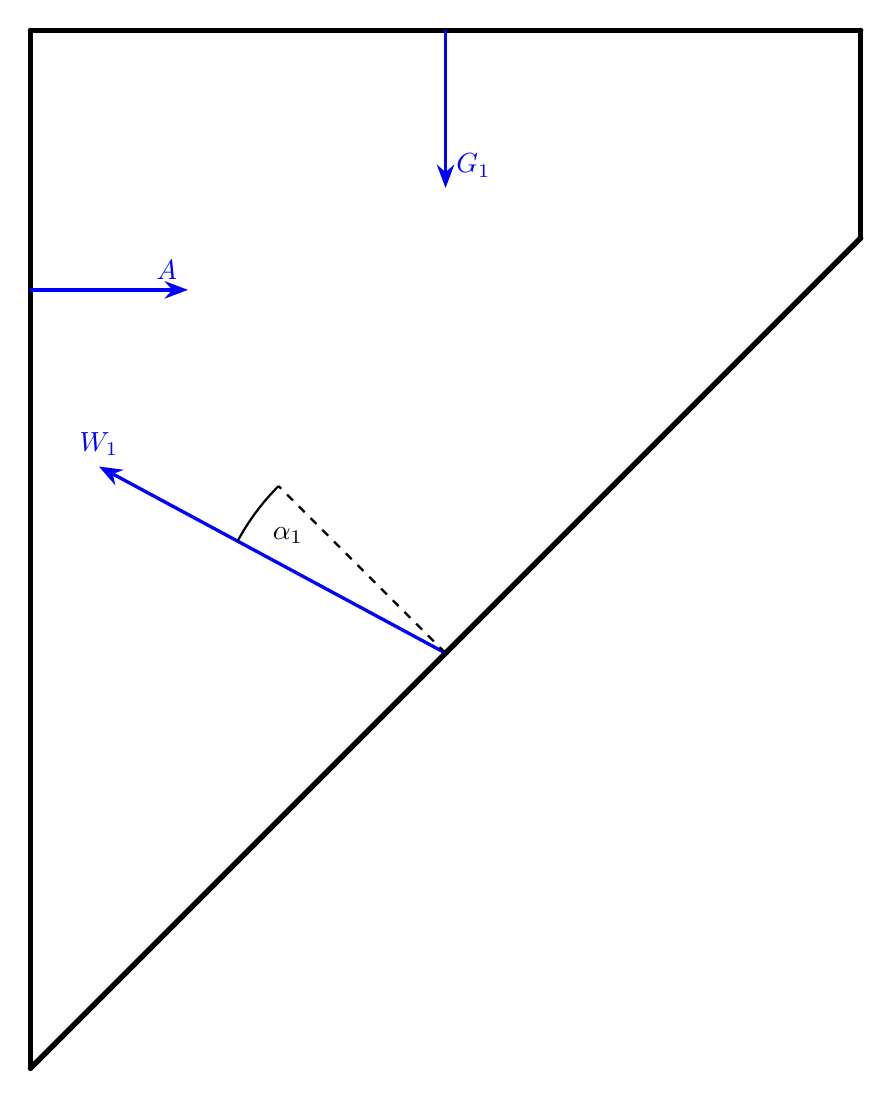
\begin{tikzpicture}[
      thick, % Default line thickness
      >=Stealth, % Default arrow tip
      force/.style={blue, very thick, ->}, % Style for force arrows
      dimline/.style={thin, <->, >=latex}, % Style for dimension lines
    ]

    % Größen
    \def\hone{1.5pt * 50}
    \def\htwo{7.5pt * 50}
    \def\w{6pt * 50}

    % Koordinaten von Punkte
    \coordinate (A) at (0, 0);
    \coordinate (B) at (\w, 0);
    \coordinate (C) at (\w, -\hone);
    \coordinate (D) at (0, -\htwo);

    % Starrkörper
    \foreach \i/\j in {A/B, B/C, C/D, D/A}
    \draw[line width=2pt, black, cap=round] (\i) -- (\j);

    % Gewichtskraft G1 (nach unten)
    \draw[force] ($(A)!0.5!(B)$) -- ++(0,-2) node[above right] {$G_1$};

    \draw[force] ($(C)!0.5!(D)$) -- ++(151.7:5cm) node[above] {$W_1$};

    \draw[dashed] ($(C)!0.5!(D)$) -- ++(135:3cm);

    % Reaktionskraft an der Wand A
    \draw[force] ($(A)!0.25!(D)$) -- ++(2,0) node[above left] {$A$};

    \coordinate (Z) at ($($(C)!0.5!(D)$) + (151.7:5cm)$);
    \coordinate (Y) at ($(C)!0.5!(D)$);
    \coordinate (X) at ($($(C)!0.5!(D)$) + (135:5cm)$) node[above, xshift=93pt, yshift=-189pt] {$\alpha_1$};
    \pic [draw, angle radius=3cm] {angle = X--Y--Z};
  \end{tikzpicture}
  \caption{Freikörperbild von Körper 1}
\end{figure}
Für Körper 1 gelten 2 Gleichgewichtsgleichungen:
\begin{align*}
  &\sum F_X = A + W_1 \cdot \cos 151,7^\circ = 0\\
  &\sum F_Y = W_1 \cdot \sin 151.7^\circ - G_1 = 0
\end{align*}
Davon:
\begin{align*}
  W_1 &= 11,601\text{ kN}\\
  A &= 10,214\text{ kN}
\end{align*}

Jetzt kann $F_{max}$ und $B$ berechnet werden.
\begin{figure}[H]
  \centering
  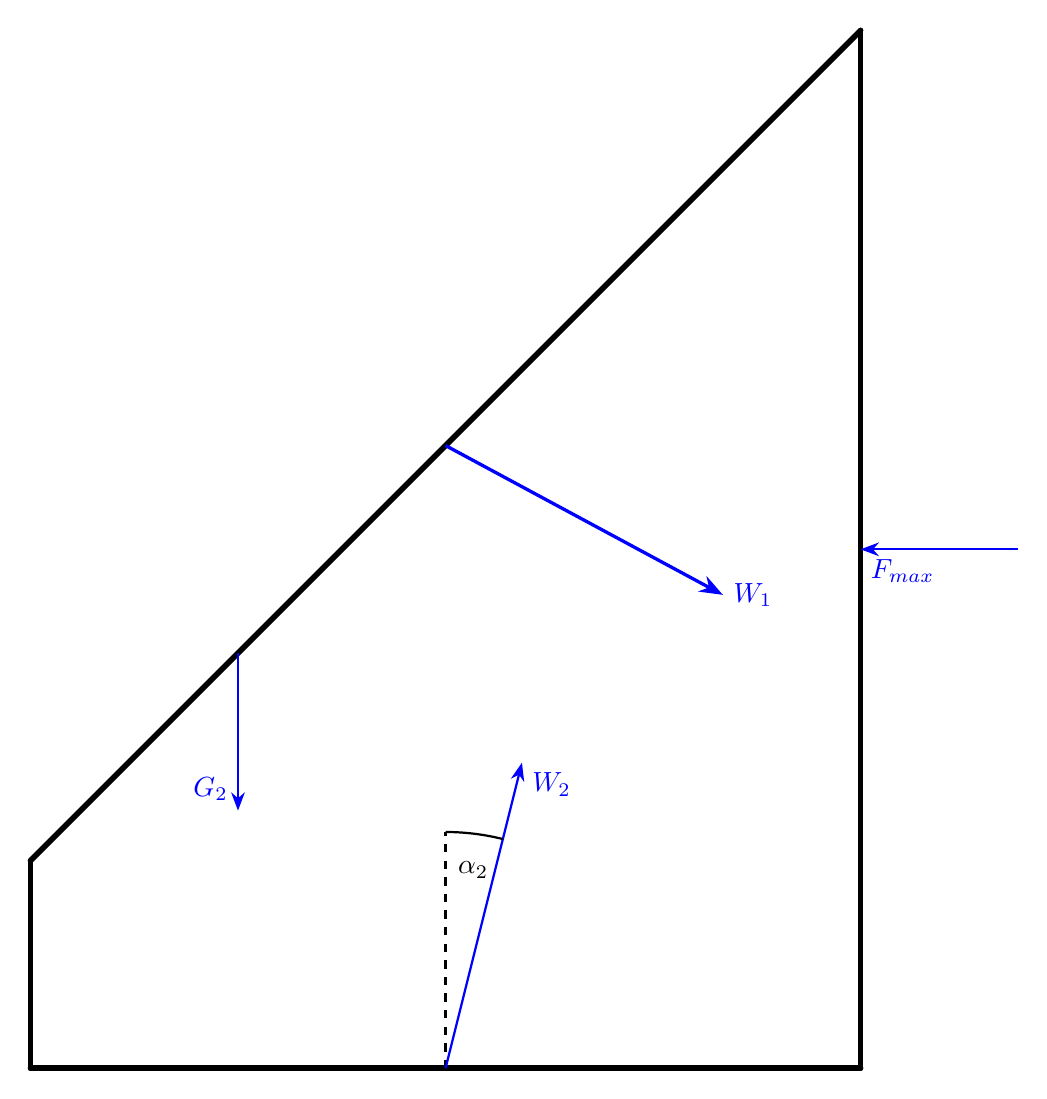
\begin{tikzpicture}[
      thick, % Default line thickness
      >=Stealth, % Default arrow tip
      force/.style={blue, very thick, ->}, % Style for force arrows
      dimline/.style={thin, <->, >=latex}, % Style for dimension lines
    ]

    % Größen
    \def\hone{1.5pt * 50}
    \def\htwo{7.5pt * 50}
    \def\w{6pt * 50}

    % Koordinaten von Punkte
    \coordinate (A) at (0, 0);
    \coordinate (B) at (\w, 0);
    \coordinate (C) at (\w, \htwo);
    \coordinate (D) at (0, \hone);

    % Starrkörper
    \foreach \i/\j in {A/B, B/C, C/D, D/A}
    \draw[line width=2pt, black, cap=round] (\i) -- (\j);

    \draw[force, thick] ($(D)!0.25!(C)$) -- ++(0,-2) node[above left] {$G_2$};

    \draw[force] ($(D)!0.5!(C)$) -- ++(331.7:4cm) node[right] {$W_1$};
    \draw[dashed] ($(A)!0.5!(B)$) -- ++(0, 3cm);
    \draw[force, thick] ($(A)!0.5!(B)$) -- ++(75.96:4cm) node[below right] {$W_{2}$};

    \draw[force, thick] ($($(B)!0.5!(C)$) + (2, 0)$) -- ++(-2,0) node[below right] {$F_{max}$};

    \coordinate (M) at ($(A)!0.5!(B)$);
    \coordinate (V) at ($(M) + (0,3cm)$);
    \coordinate (W2) at ($(M) + (75.96:4cm)$) node[above, xshift=160pt, yshift=65pt] {$\alpha_2$};
    \pic[draw, angle radius=3cm] {angle = W2--M--V};

  \end{tikzpicture}
  \caption{Freikörperbild von Körper 2}
\end{figure}
Für Körper 2 gelten auch 2 Gleichgewichtsgleichungen.
\begin{align*}
  &\sum F_X = W_1 \cdot \cos (-28,3)^\circ + W_2 \cdot \cos 75,96^\circ - F_{max} = 0\\
  &\sum F_Y = W_1 \cdot \sin (-28,3)^\circ + W_2 \cdot \sin 75,96^\circ- G_2 = 0
\end{align*}
Davon:
\begin{align*}
  &W_2 = 8,246\text{ kN} = B \\
  &F_{max} = 12,214\text{ kN}
\end{align*}

\section[Gleichgewichtzustand]{Gleichgewichtanalyse im Fall $\mu_1 = 0$ und $F = c_1G_1 + c_2G_2$}
\begin{align*}
  F = c_1 \cdot G_1 + c_2 \cdot G_2 = 6,05\text{ kN}
\end{align*}
Unbekannt ist $A$ und $\tilde{B}$. $\tilde{B}$ wird berechnet. Wenn die Winkel dieser Kraft kleiner ist als die Haftungwinkel $\alpha_2$, ist das Kraftsystem im Gleichgewicht.

$W_1$ wird gleich Groß sein als $N_1$ in diesem Fall, weil wegen $\mu_1 = 0$ $H_1$ null ist.
\begin{figure}[H]
  \centering
  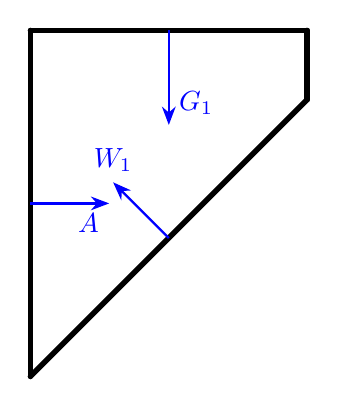
\begin{tikzpicture}[
      thick, % Default line thickness
      >=Stealth, % Default arrow tip
      force/.style={blue, very thick, ->}, % Style for force arrows
      dimline/.style={thin, <->, >=latex}, % Style for dimension lines
    ]

    % Größen
    \def\hone{0.5pt * 50}
    \def\htwo{2.5pt * 50}
    \def\w{2pt * 50}
    \def\fg{5.5pt * 2 / 3}
    \def\fa{4ptpt * 2 / 3}

    % Koordinaten von Punkte
    \coordinate (A) at (0, 0);
    \coordinate (B) at (\w, 0);
    \coordinate (C) at (\w, -\hone);
    \coordinate (D) at (0, -\htwo);

    % Starrkörper
    \foreach \i/\j in {A/B, B/C, C/D, D/A}
    \draw[line width=2pt, black, cap=round] (\i) -- (\j);

    % Gewichtskraft G1 (nach unten)
    \draw[force, thick] ($(A)!0.5!(B)$) -- ++(0,-1.2) node[above right] {$G_1$};

    % Kontaktkraft N12: normale zur 45°-Fläche
    % Richtung: von Körper 2 auf Körper 1 → wirkt nach oben-links
    \draw[force, thick] ($(C)!0.5!(D)$) -- ++(135:1)
    node[above] {$W_{1}$};

    % Reaktionskraft an der Wand A
    \draw[force, thick] ($(A)!0.5!(D)$) -- ++(1,0) node[below left] {$A$};
  \end{tikzpicture}
  \caption{Freikörperbild von Körper 1}
\end{figure}
$W_1$ wird auf Komponente $W_{1X}$ und $W_{1Y}$ zerlegt so, dass $W_{1X} = W_{1Y}$. Die zwei Gleichgewichtsgleichungen:
\begin{align*}
  &\sum F_X = A + W_{1X} = 0\\
  &\sum F_Y = G_1 + W_{1Y} = 0\\
\end{align*}
Davon:
\begin{align*}
  &W_{1X} = W_{1Y} = 5,5\text{ kN}\\
  &A = 5,5\text{ kN}
\end{align*}
Jetzt können die Gleichungen für Körper 2 aufgeschrieben werden.
\begin{figure}[H]
  \centering
  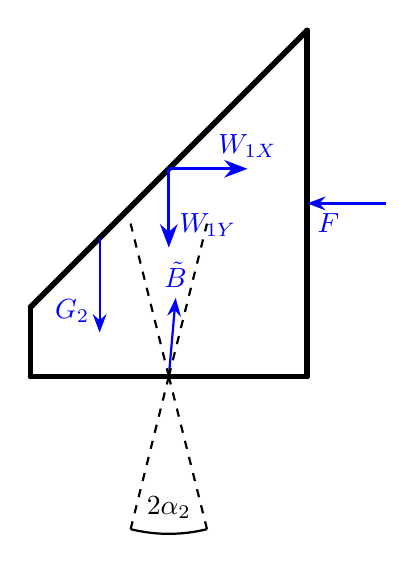
\begin{tikzpicture}[
      thick, % Default line thickness
      >=Stealth, % Default arrow tip
      force/.style={blue, very thick, ->}, % Style for force arrows
      dimline/.style={thin, <->, >=latex}, % Style for dimension lines
    ]

    % Größen
    \def\hone{0.5pt * 50}
    \def\htwo{2.5pt * 50}
    \def\w{2pt * 50}
    \def\fg{5.5pt * 2 / 3}
    \def\fa{4ptpt * 2 / 3}

    % Koordinaten von Punkte
    \coordinate (A) at (0, 0);
    \coordinate (B) at (\w, 0);
    \coordinate (C) at (\w, \htwo);
    \coordinate (D) at (0, \hone);

    % Starrkörper
    \foreach \i/\j in {A/B, B/C, C/D, D/A}
    \draw[line width=2pt, black, cap=round] (\i) -- (\j);

    \draw[force, thick] ($(D)!0.25!(C)$) -- ++(0,-1.2) node[above left] {$G_2$};

    \draw[force] ($(D)!0.5!(C)$) -- ++(0:1cm) node[above] {$W_{1X}$};
    \draw[force] ($(D)!0.5!(C)$) -- ++(-90:1cm) node[above right] {$W_{1Y}$};

    \draw[force, thick] ($(A)!0.5!(B)$) -- ++(85:1cm)
    node[above] {$\tilde{B}$};
    \draw[force, thick] ($($(B)!0.5!(C)$) + (1, 0)$) -- ++(-1,0) node[below right] {$F$};

    \draw[dashed] ($(A)!0.5!(B)$) -- ++(75.96:2cm);
    \draw[dashed] ($(A)!0.5!(B)$) -- ++(104.04:2cm);
    \draw[dashed] ($(A)!0.5!(B)$) -- ++(255.96:2cm);
    \draw[dashed] ($(A)!0.5!(B)$) -- ++(284.04:2cm);

    \coordinate (X) at ($(\w / 2, 0) + (255.96:2cm)$);
    \coordinate (Y) at (\w / 2, 0);
    \coordinate (Z) at ($(\w / 2, 0) + (284.04:2cm)$) node[above, xshift=50pt, yshift=-55pt] {$2\alpha_2$};
    \pic [draw, angle radius=2cm] {angle = X--Y--Z};

  \end{tikzpicture}
  \caption{Freikörperbild von Körper 2}
\end{figure}
\begin{align*}
  &\sum F_X = W_{1X} - F + \tilde{B}_X = 0\\
  &\sum F_Y = G_2 - W_{1Y} + \tilde{B}_Y = 0\\
\end{align*}
Nach der Lösüng bekommt:
\begin{align*}
  &\boxed{\tilde{B}_X = -0,55\text{ kN}}\\
  &\boxed{\tilde{B}_Y = 8\text{ kN}}\\
  &\boxed{\tilde{B} = \sqrt{\tilde{B}_X^2 + \tilde{B}_Y^2} = 8,019\text{ kN}}
\end{align*}

Die Winkel $\beta$ von $\tilde{B}$ ist:
\begin{align*}
  &\beta = \tan \frac{\tilde{B}_X}{\tilde{B}_Y}\\
  &\boxed{\beta = 3,933^\circ}
\end{align*}

Die maximale Haftungswinkel von $\tilde{B}$ ist $14,04^\circ$. Weil $\beta$ kleiner ist, wird das Kraftsystem nicht bewegen, also ist im Gleichgewicht.
\end{document}
